\section{Versuchsablauf}

\rule{\linewidth}{0.5mm}
\subsection{Der Versuch}
\begin{addmargin}[3cm]{0cm}
	In diesem Praktikum soll die Gesamt-, die Carbonat- und die Nichtcarbonathärte von
	
	\begin{itemize}
		\item Leitungswasser
		
		\item Leitungswasser nach Brita-Filter
		
		\item Leitungswasser nach Kalkex 5000
	\end{itemize}
	
	bestimmt werden.
	
	\begin{figure}[H]\centering
		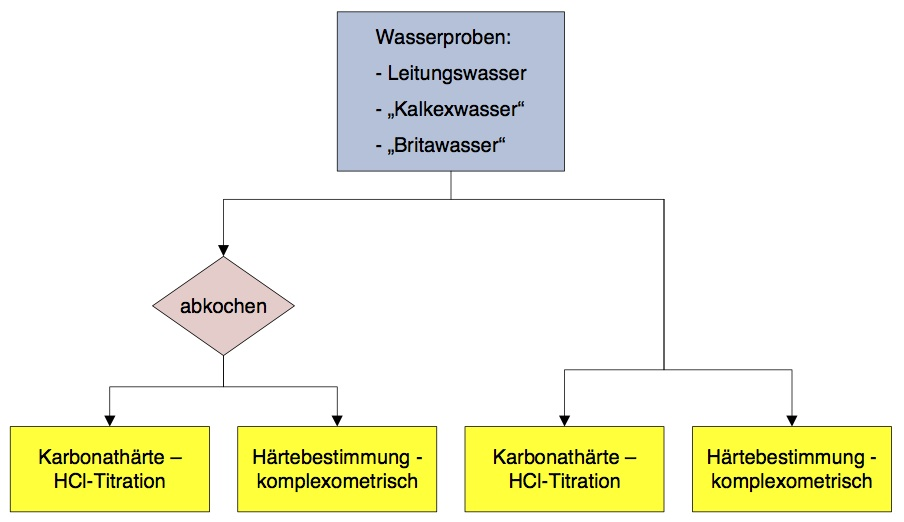
\includegraphics[scale=0.7]{./pictures/uebersichtVersuch.jpg}
		\caption{Übersicht für den Ablauf des Versuches}
		\label{Ablauf}
	\end{figure}
\end{addmargin}


\rule{\linewidth}{0.5mm}
\subsection{Wasser bereitstellen}
\begin{addmargin}[3cm]{0cm}
	\begin{enumerate}
		\item Je Probestelle 20 - 30l in den Abguss fliessen lassen
		
		\item Je Probestelle 2l Wasser für den Versuch bereitstellen
		
		\item \begin{itemize}
					\item	Je Probe 200ml Probewasser und 2 Siedesteinchen mittels Pinzette in einem 250ml-Erlenmeyer-kolben mit Schliff geben und während einer Stunde am Rückflusskühler kochen.
					
					\item	Dies soll aus Zeitgründen so schnell wie möglich geschehen.
					
					\item Darauf achten, dass jede Probe exakt gleich lang kocht
					
					\item Temperatureinstellung: $310^\circ$C
			  \end{itemize}
	\end{enumerate}
	
\end{addmargin}

\rule{\linewidth}{0.5mm}
\subsection{Komplexometrische Härtebestimmung}
\begin{addmargin}[3cm]{0cm}
	\begin{enumerate}
		\item Glas des Titrierautomaten mit deionisiertem Wasser sauber spülen
	
		\item 50ml Probenwasser mit Vollpipette in das Glas geben
		
		\item Probenwasser mit 10ml Pufferlösung und 1ml Eriochromschwarz-Lösung versetzen
		
		\item Glas mit der Probe am Titrierautomaten befestigen und Messung starten
		
		\item Verbrauch an 0.1$\frac{\mathrm{mol}}{\mathrm{l}}$ Titriplex(EDTA)-Lösung ablesen und notieren(in ml).
	\end{enumerate}
	\vspace{0.5cm}
	Der Endpunkt des Titrierens äussert sich durch einen sprunghaften Farbumschlag, welcher dann stattfindet, wenn dem Indikatorfarbkomplex alle Metallionen entzogen wurden. Dies passiert weil die Metallionen mit dem EDTA eine stabilere Komplexverbindung eingehen als mit dem Eriochromschwarz-Farbkomplex. An jedes $\chemfig{Ca^{2+}}$- und $\chemfig{Mg^{2+}}$-Ion wird je ein Komplexonion gebunden, also entspricht die Gesamthärte genau der Konzentration an Komplexonionen beim Farbwechsel. Dieser Farbwechsel wird vom Titrierautomaten detektiert und die verbrauchte Menge an EDTA-Lösung angezeigt.
	
	\vspace{0.5cm}
	
	$\boxed
	{
		\begin{aligned}
			V_{Komp} &= \text{Verbrauchtes Volumen an Titriplex(EDTA)-Lösung} \\
			c_{Komp} &= 0.1 \frac{\mathrm{mol}}{\mathrm{l}}= \text{Konzentration der Titriplex(EDTA)-Lösung} \\
			V_{W} &= 50ml = \text{Volumen des Probenwassers} \\
			n_{Komp} &= V_{Komp}\cdot c_{Komp} =\text{Molmenge der Verbrauchten Titriplex(EDTA)-Lösung} \\
			\mathrm{GH} &=   \frac{n_{Komp}}{V_{Komp}+V_{W}} 
		\end{aligned}
	}$
	
	\vspace{0.5cm}
\end{addmargin}

\rule{\linewidth}{0.5mm}
\subsection{Hydrogencarbonatbestimmung durch Neutralisation mit Salzsäure}
\begin{addmargin}[3cm]{0cm}
		\begin{enumerate}
			\item 100ml Probewasser mit einer Vollpipette in einen 250ml Erlenmeyerkolben pipettieren
		
			\item Rührmagneten dazugeben
			
			\item 2 Tropfen Mischindikator dazugeben
			
			\item Tropfenweise mit 0.1$\frac{\mathrm{mol}}{\mathrm{l}}$ $\chemfig{HCl}$-Lösung bis zum Farbumschlag von blaugrün nach hellrosa titrieren.
		\end{enumerate}
		
		\vspace{0.5cm}
		$\boxed
		{
			\begin{aligned}
				V_{\mathrm{HCl}} &= \text{Verbrauchtes Volumen an } \chemfig{HCl} \text{-Lösung} \\
				c_{\mathrm{HCl}} &= 0.1 \frac{\mathrm{mol}}{\mathrm{l}}= \text{Konzentration der } \chemfig{HCl} \text{-Lösung} \\
				V_{W} &= 100ml = \text{Volumen des Probenwassers} \\
				n_{\mathrm{HCl}} &= V_{\mathrm{HCl}}\cdot c_{\mathrm{HCl}} =\text{Molmenge der Verbrauchten } \chemfig{HCl} \text{-Lösung} \\
				\mathrm{KH} &=   \frac{1}{2}\cdot c(\chemfig{HCl}) = \frac{1}{2}\cdot \frac{n_{\mathrm{HCl}}}{V_{\mathrm{HCl}}+V_{W}} 
			\end{aligned}
		}$
		
		\vspace{0.5cm}
\end{addmargin}


\rule{\linewidth}{0.5mm}
\subsection{Gesamthärtebestimmung mittels Schnelltest}
\begin{addmargin}[3cm]{0cm}
		Teststäbchen eintauchen, Wert ablesen, nach dem Trocknen ins Journal kleben.
\end{addmargin}

\rule{\linewidth}{0.5mm}
\subsection{Beurteilung der Wirkung des Kalkex 5000}
\begin{addmargin}[3cm]{0cm}
		Es soll aufgrund des weissen Niederschlags, der beim Abkochen an den Gefässwänden entstand, diskutiert werden, ob die Behandlung des Wassers durch den Kalkex 5000 eine Wirkung zeigte. Laut Herstellerangaben sollte sich die Kristallstruktur von Kalk und somit die Kalkausfällung qualitativ verändern.
\end{addmargin}
